\chapter{基本概念}
\section{何谓量子}
\begin{center}
    \itshape
    “场的最小激发是量子。” \\
    “量子代表了一种观点，即：‘世界不是连续的，而是分立的’。”
\end{center}

\section{一点历史}
\subsection{黑体辐射}
使用经典理论给出公式的Wein、Rayleigh和Jeans都失败了。
Rayleigh-Jeans公式以能量按自由度均分定理为基础：
\begin{equation}
    I(\omega) = \dfrac{\omega^2}{\pi^2 c^2}kT
\end{equation}
在$\omega$较大时快速发散，即\textcolor{PurpleDeep}{\textbf{紫外灾难}}。

Planck以插值法通过Wien公式和Rayleigh-Jeans公式拟合得到了Plunck公式。
\begin{derivation}
    \[
        I(w) = \dfrac{1}{\textcolor{PurpleDeep}{e^{a\omega/kT}}-1} \cdot \dfrac{b\omega^3}{\pi^2 c^2}\quad a,b\text{为常数}
    \]
    Planck发现$\textcolor{PurpleDeep}{e^{a\omega/kT}}$形似Bolztmann分布$N_n = N_1 e^{-(E_n-E_1)/kT}$。
    
    因此，他假设\textbf{辐射场中偶极振子的能量是一份一份的，每份能量依赖于角频率}。
    \begin{equation*}
        E = a\omega \qquad N_n = N_0 e^{-E_n/kT} = N_0 e^{-na\omega/kT}
    \end{equation*}
    平均能量：
    \begin{align*}
        \langle E \rangle &= \frac{\sum_{n} N_n \cdot E_n}{\sum_{n} N_n} \\[1ex]
        &= \frac{\sum_{n} N_0 e^{-na\omega/kT} \cdot na\omega}{\sum_{n} N_0 e^{-na\omega/kT}} \\[1ex]
        &= \frac{a\omega (0 \cdot e^{-0/kT} + 1 \cdot e^{-1a\omega/kT} + 2 \cdot e^{-2a\omega/kT} + \cdots)}{e^{-0/kT} + e^{-1a\omega/kT} + e^{-2a\omega/kT} + \cdots} \\[1ex]
        &\xlongequal{\varepsilon = e^{-a\omega/kT}} \frac{a\omega (\varepsilon + 2\varepsilon^2 + 3\varepsilon^3 + \cdots)}{1 + \varepsilon + \varepsilon^2 + \varepsilon^3 + \cdots} \\[1ex]
        &= \frac{a\omega \varepsilon \frac{d}{d\varepsilon} (1 + \varepsilon + \varepsilon^2 + \varepsilon^3 + \cdots)}{1 + \varepsilon + \varepsilon^2 + \varepsilon^3 + \cdots} \\[1ex]
        &\xlongequal{\text{Taylor 展开}} \frac{a\omega \varepsilon \frac{d}{d\varepsilon} (\frac{1}{1-\varepsilon})}{\frac{1}{1-\varepsilon}} \\[1ex]
        &= a\omega \varepsilon \frac{1}{1-\varepsilon} = a\omega \frac{e^{-a\omega/kT}}{1 - e^{-a\omega/kT}} \\[1ex]
        &= a\omega \frac{1}{e^{a\omega/kT} - 1}
    \end{align*}
    Rayleigh-Jeans 公式中的能量项为$kT$，用$\langle E \rangle$取代之：
    \[
    I(\omega) = \frac{\omega^2}{\pi^2 c^2} \textcolor{PurpleDeep}{kT} = \frac{\omega^2}{\pi^2 c^2} \cdot \textcolor{PurpleDeep}{a\omega \frac{1}{e^{a\omega/kT} - 1}} = \frac{1}{e^{a\omega/kT} - 1} \frac{a\omega^3}{\pi^2 c^2}
    \]
    这就是Plunck公式，式中$a$即为如今的$\hbar $。
\end{derivation}

\subsection{光电效应}
Einstein基于Planck的假说，提出光是一份一份的\overtext{能量子}{energy quantum}/\overtext{光量子}{light quantum}构成的，每个光子的能量$E=h\nu=\hbar\omega$。
\[
    E^2=m^2c^4=m_0^2c^4+(pc)^2 \xlongequal{\text{光量子}m_0=0}p^2c^2 \Rightarrow  E = pc \Rightarrow p = \frac{h\mu}{c}=\frac{h}{\lambda}
\]

\subsection{Comptom效应}

\subsection{de Brogile波}

\section{Schrödinger方程}
\subsection{Schrödinger方程的推导}
\begin{derivation}
    Schrödinger根据光的波动性和de Brogile的波粒二象性猜测出了实物粒子的波动方程：
    \[\varphi(x,t) = A\cos(kx-\omega t)\]
    根据Euler公式$e^{i\theta} = \cos\theta + i\sin\theta$有：
    \[\varphi(x,t) = A\text{Re}\{e^{i(kx-\omega t)}\}\]
    为了便于数学处理，用整个复数表示波：
    \[\varphi(x,t) = Ae^{i(kx-\omega t)}\]
    实物粒子$E = \hbar\omega \Rightarrow k = \frac{2\pi}{\lambda} = \frac{p}{\hbar}$代入上式中，于是有自由实物粒子的波动方程：
    \[\psi(x,t) = Ae^{\frac{i}{\hbar}(px-Et)}\]
    考察波函数关于t的变化：
    \[\frac{\partial}{\partial t}\psi = -\frac{i}{\hbar}EAe^{\frac{i}{\hbar}(px-Et)} \Rightarrow \textcolor{PurpleDeep}{i\hbar\frac{\partial}{\partial t}\psi=E\psi}\]
    考察波函数关于x的变化，为了获取能量项，取二阶导：
    \[\frac{\partial^2}{\partial x^2}\psi = \left(-\frac{p}{i\hbar}\right)^2 Ae^{\frac{i}{\hbar}(px-Et)} = \left(-\frac{1}{i\hbar}\right)^2 2\mu E\psi \Rightarrow \textcolor{PurpleDeep}{\frac{1}{2\mu}\left(-i\hbar\frac{\partial}{\partial x}\right)^2 \psi = E\psi}\]
    联立上述二式：
    \[i\hbar\frac{\partial}{\partial t}\psi = \frac{1}{2\mu}\left(-i\hbar\frac{\partial}{\partial x}\right)^2 \psi = E\psi\]
    这就是Schrödinger方程
\end{derivation}
事实上，Schrödinger作上述推导\textbf{纯粹基于猜想}，没有严密的数学推导，它在量子力学中是作为公理存在的。

\subsection{Born统计诠释}
\begin{center}
    \textit{波函数$\psi$的意义是什么？}
    
    \textit{到底是什么在波动？}
\end{center}

Born类比光波的模平方等于光强，即光子在该处的密度大小，故而对实物粒子，\textbf{波函数的模平方表示实物粒子出现在该处的概率密度大小}

因此有\textbf{归一化条件}：
\[\int_{-\infty }^{+\infty}|\psi|^2 \dd{\tau } = 1\]

而波函数本身是概率振幅，是概率的平方根，没有实际意义。

\section{电子双缝干涉实验}
\subsection{电子是如何穿过双缝的？}
电子以概率波的形式同时穿过两缝并产生干涉，落到光屏上又坍缩为粒子。
\begin{derivation}
    设电子通过缝$1$的状态为$\psi_1$，通过缝$2$的状态为$\psi_2$，这种某个量确定的态称为\textbf{本征态}。

    \noindent \textbf{若不施以观测：}

    通过双缝后的粒子处于叠加态:
    \[\psi = c_1\psi_1 + c_2\psi_2 \quad \text{(概率振幅叠加)} \qquad \text{归一化条件：}|c_1|^2 + |c_2|^2 = 1\]
    概率密度：
    \[\begin{aligned}
        \rho = |\psi|^2 = \psi^* \cdot \psi &= (C_1^* \psi_1^* + C_2^* \psi_2^*)(C_1 \psi_1 + C_2 \psi_2) \\ 
        &= |C_1|^2 |\psi_1|^2 + |C_2|^2 |\psi_2|^2 + \textcolor{PurpleDeep}{C_1^* C_2 \psi_1^* \psi_2 + C_1 C_2^* \psi_1 \psi_2^*} \\
        &= |C_1|^2 |\psi_1|^2 + |C_2|^2 |\psi_2|^2 + \textcolor{PurpleDeep}{2 \text{Re} \{ C_1^* C_2 \psi_1^* \psi_2 \}} \\
        &= |C_1|^2 |\psi_1|^2 + |C_2|^2 |\psi_2|^2 + \textcolor{PurpleDeep}{2 \text{Re} \{ |C_1| |\psi_1| e^{-i\theta_1} \cdot |C_2| |\psi_2| e^{i\theta_2} \}} \\
        &= |C_1|^2 |\psi_1|^2 + |C_2|^2 |\psi_2|^2 + \textcolor{PurpleDeep}{2 |C_1| |\psi_1| |C_2| |\psi_2| \cos(\theta_2 - \theta_1)} \\
        &= |C_1|^2 |\psi_1|^2 + |C_2|^2 |\psi_2|^2 + \textcolor{PurpleDeep}{\underbrace{2 |C_1| |\psi_1| |C_2| |\psi_2| \cos \theta}_{\text{干涉项}}}
    \end{aligned}\]

    \noindent \textbf{若施以观测：}

    粒子在经过探测器后发生坍缩，落入某个本征态，干涉花样消失。
    \begin{align*}
    \psi = C_1\psi_1 + C_2\psi_2
    \begin{cases} 
        \text{以 } |C_1|^2 \text{ 的概率坍缩到 } \psi_1 \\
        \text{以 } |C_2|^2 \text{ 的概率坍缩到 } \psi_2
    \end{cases} \\
    \text{总强度}\quad I = I_1 + I_2 = \underbrace{|C_1|^2 |\psi_1|^2 + |C_2|^2 |\psi_2|^2}_{\text{无干涉项}}
    \end{align*}
\end{derivation}
以上内容被称为\textbf{态叠加原理/测量假设}。

实验现象表明：

\begin{itemize}
\item \textbf{一旦确定了电子从哪个缝通过，就会破坏掉干涉花样。}
    \begin{mistake}
        注意，“观测”不是一个唯心的过程，而是粒子的位置信息与外部环境发生纠缠的过程，不以人的意志为转移。
    \end{mistake}
\item \textbf{电子路径的精确度越大，干涉花样的精确度越小。} \\
这是一个粗略版的\overtext{不确定性原理}{uncertainty principle}。
\end{itemize}

\subsection{延迟选择实验}
\overtext{延迟选择}{delay-selection}实验表明，在电子通过狭缝后再加上探测器仍会使干涉花样消失。

\subsection{概率振幅解释}
把粒子出现在$x$处这一位置的本征态记为$\ket{x}$，粒子处于态$\ket{\psi}$。

记“在$\ket{\psi}$态中找到粒子处于$\ket{x}$本征态”为$\langle x | \psi \rangle$，那么$\psi(x) = \langle x | \psi \rangle$，概率密度$\rho = |\langle x | \psi \rangle|^2$

\begin{minipage}[t]{0.35\textwidth} % 左侧放图片
    \vspace{0pt} % 关键：确保顶端对齐
    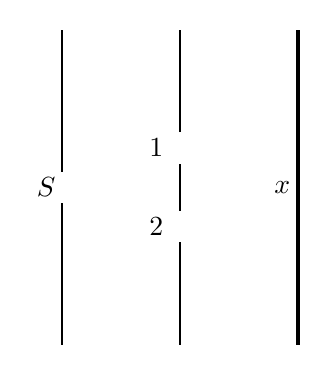
\begin{tikzpicture}[thick, >=stealth]
        \node at (0.3, 1.5) {$S$};
        \draw (0.5,-0.5) -- (0.5,1.3) (0.5,1.7) -- (0.5,3.5);
        % 第一个挡板
        \draw (2,-0.5) -- (2,0.8) (2,1.2) -- (2,1.8) (2,2.2) -- (2,3.5);
        \node at (1.7, 2) {$1$};
        \node at (1.7, 1) {$2$};
        \draw[ultra thick] (3.5,-0.5) -- (3.5,3.5); % 屏幕
        \node at (3.3, 1.5) {$x$};
    \end{tikzpicture}
\end{minipage}
\begin{minipage}[t]{0.5\textwidth} % 右侧放文字
    \vspace{0pt}
    \textbf{若只有一个双缝挡板：}\\
    电子经由$S$打到屏上$x$处总的概率幅：
    \[\langle x|s \rangle = \langle x|1 \rangle \langle 1|s \rangle + \langle x|2 \rangle \langle 2|s \rangle\]
    即$\psi = c_1 \psi_1 + c_2 \psi_2$
\end{minipage}

\vspace{1em}

\begin{minipage}[t]{0.35\textwidth} % 左侧放图片
    \vspace{0pt} % 关键：确保顶端对齐
    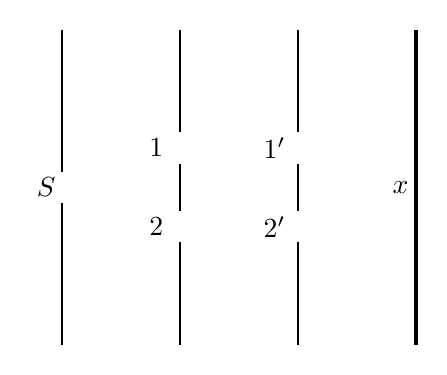
\begin{tikzpicture}[thick, >=stealth]
        \begin{scope}[yshift=-5cm]
            \node at (0.3, 1.5) {$S$};
            \draw (0.5,-0.5) -- (0.5,1.3) (0.5,1.7) -- (0.5,3.5);
            % 第一个挡板
            \draw (2,-0.5) -- (2,0.8) (2,1.2) -- (2,1.8) (2,2.2) -- (2,3.5);
            \node at (1.7, 2) {$1$};
            \node at (1.7, 1) {$2$};
            % 第二个挡板
            \draw (3.5,-0.5) -- (3.5,0.8) (3.5,1.2) -- (3.5,1.8) (3.5,2.2) -- (3.5,3.5);
            \node at (3.2, 2) {$1'$};
            \node at (3.2, 1) {$2'$};
            % 屏幕
            \draw[ultra thick] (5,-0.5) -- (5,3.5);
            \node at (4.8,1.5) {$x$};
        \end{scope}
    \end{tikzpicture}
\end{minipage}
\begin{minipage}[t]{0.55\textwidth} % 右侧放文字
    \vspace{0pt}
    \textbf{若有两个双缝挡板：}
    \begin{align*}
        \langle x|s \rangle =& \langle x|1' \rangle \langle 1'|1 \rangle \langle 1|s \rangle + \langle x|1' \rangle \langle 1'|2 \rangle \langle 2|s \rangle \\
        +& \langle x|2' \rangle \langle 2'|1 \rangle \langle 1|s \rangle + \langle x|2' \rangle \langle 2'|2 \rangle \langle 2|s \rangle
    \end{align*}    
\end{minipage}
\vspace{1em}

\textbf{若两个挡板上开n个缝：}
\[\langle x|s \rangle = \sum_{i}^n \sum_{j}^n \langle x|i \rangle \langle i|j \rangle \langle j|s \rangle\]

\textbf{若有m个挡板上开n个缝：}
\[\langle x|s \rangle = \underbrace{\sum_i^n \sum_j^n \sum_k^n \dots \sum_?^n}_{m \text{个求和}} \langle x|i \rangle \langle i|j \rangle \langle j| \dots |? \rangle \langle ?|s \rangle\]

若$m \rightarrow \infty, n \rightarrow \infty$则遍历了整个空间，即自由空间中电子自$S$到挡板上$x$处的概率幅$\langle x|s \rangle$与所有可能路径有关。这就是\overtext{路径积分}{path integral}的基础概念。

\section{Schrödinger's Cat}
Schrödinger's Cat是Schrödinger设计的\textbf{思想实验}，用以批驳Copenhagen诠释不符合物理直觉，至今仍是量子力学领域的试金石。

\section{Bohr原子模型}
Bohr之前，有J.J.Thompson的\textbf{枣糕模型}和Rutherford的\textbf{行星模型}。
早在1915年，Schrödinger方程提出之前(1925)，Bohr创新性地基于Rutherford行星模型、Planck能量分立假说、Einstein光子说和氢光谱经验公式$\tilde{v}(m,n) = R_{\mathrm H}\left(\frac{1}{m^2}-\frac{1}{n^2}\right)$提出了\textbf{Bohr原子模型}

\subsection{Bohr原子模型的三大假设}
\begin{itemize}
    \item \textbf{定态假设}\\
    电子绕核作圆周运动时只能在一些分立的轨道上，并具有稳定的能量，即不向外辐射电磁波。
    \item \textbf{辐射条件}\\
    当原子中的电子从一个定态n跃迁至定态m时会以电磁波的形式放出/吸收能量。
    \item \textbf{角动量量子化}
    \begin{gather*}
        L = m_e vr = n\hbar \Rightarrow E_n = -\frac{hcR_{\mathrm{H}}}{n^2} \\
        h\nu_{m \rightarrow n} = E_n - E_m \Rightarrow \nu_{m \rightarrow n} = cR_{\mathrm H}\left(\frac{1}{m^2}-\frac{1}{n^2}\right)
    \end{gather*}
\end{itemize}

\subsection{Bohr原子模型的缺陷}
通过强行假定克服能量不守恒的问题，且只适用于氢原子与类氢原子，对多电子体系无效。

\section{矩阵力学}
矩阵力学是由Heisenberg独立地提出的量子力学等价形式。

\subsection{实证主义}
Heisenberg主张整个量子力学应以\overtext{可观测量/力学量}{observable}为基础。

Bohr理论的“轨道”不具备物理意义，而能级差是可观测的，有物理意义。

描述能级差需基于初、末两个状态共同决定，描述一个状态需要一系列数，因此可观测量应当是一个二维方阵，表达了状态的变化。

\subsection{矩阵与算符}
\begin{itemize}
    \item \textbf{从具象视角来看：} \\
    Heisenberg利用\overtext{矩阵}{matrix}表达状态的改变方式，用一维列矩阵表示一个态。
    \item \textbf{从抽象视角来看：} \\
    矩阵作为\overtext{算符}{operator}，对应了一种观测(操作)，作用是使一个态转换成另一个态。
    \begin{gather*}
        \begin{bmatrix} \hat{O} \end{bmatrix} 
        \begin{bmatrix} \psi \end{bmatrix} = 
        \begin{bmatrix} \psi' \end{bmatrix} \qquad
        \text{可记作 } \hat{O} |\psi\rangle = |\psi'\rangle
    \end{gather*}
    这是一种线性代数的语言。
\end{itemize}

\section{线性代数基础}
\subsection{线性矢量空间(LVS)}
\begin{definition}
    \overtext{线性矢量空间}{linear vector space} $\mathbb{V}$ 是由众多矢量$\ket{v_i}$构成的集合。
\end{definition}
LVS满足如下法则：
\begin{enumerate}
    \item \textbf{封闭性} \\
    矢量空间中任意矢量的线性组合仍在该矢量空间中。
    \item \textbf{数乘的分配律}
    \begin{gather*}
        a ( |v_1\rangle + |v_2\rangle ) = a |v_1\rangle + a |v_2\rangle \\
        (a + b) |v\rangle = a |v\rangle + b |v\rangle
    \end{gather*}
    \item \textbf{矢量和交换律}
    \[|v_1\rangle + |v_2\rangle = |v_2\rangle + |v_1\rangle\]
    \item \textbf{矢量和结合律}
    \[|v_1\rangle + ( |v_2\rangle + |v_3\rangle ) = ( |v_1\rangle + |v_2\rangle ) + |v_3\rangle\]
    \item \textbf{零矢量存在性} \\
    存在一个零矢量对任意矢量都满足$|0\rangle + |v\rangle = |v\rangle$，即$|0\rangle = 0 |v\rangle$。
    \item \textbf{逆矢量存在性} \\
    对任意矢量$\ket{v}$都存在$\ket{-v}$使$|v\rangle + |-v\rangle = |0\rangle$，即$|-v\rangle = - |v\rangle$。
\end{enumerate}

反直觉的是，如所有的$2\times 2$矩阵、定义在$(a,b)$上的所有函数$\{f\}$等“不那么矢量”的东西也满足LVS的定义。

也就是说：

\textbf{LVS中的元素不需要大小和方向。}

\begin{definition}
    构造矢量空间$\mathbb{V}$时所用到的所有可能的组合系数$a$所在的空间称为$\mathbb{V}$的\textbf{基域}。
    \[
    \mathbb{V}\text{的基域}
    \begin{cases}
        \text{由所有实数组成} \rightarrow \mathbb{V}\text{为实矢量空间} \\
        \text{由所有复数组成} \rightarrow \mathbb{V}\text{为复矢量空间}
    \end{cases}
    \]
\end{definition}

\begin{definition}
    线性相关性
\end{definition}

\begin{definition}
    若一个LVS最多容纳$n$个线性无关的矢量，则称该空间为$n$维的。
\end{definition}

\begin{definition}
    将$n$维空间中的$n$个线性无关的矢量称作该矢量空间的一组\overtext{基}{base}。
\end{definition}
一般来说，基不是唯一的。

\begin{definition}
    矢量在基下的展开系数称为其在这组基下的\overtext{分量}{component}。
\end{definition}
对于给定的基，同一矢量的分量是唯一的。

\subsection{内积空间(IPS)}
传统的矢量内积$\vec{A} \cdot \vec{B} = |\vec{A}| |\vec{B}| \cos\theta = \sum_{i}^n a_i b_i$具有如下性质：
\begin{itemize}
    \item $\vec{A} \cdot \vec{B} = \vec{B} \cdot \vec{A}$
    \item $\vec{A} \cdot \vec{A} \ge 0$
    \item $\vec{A} \cdot (b\vec{B} + c\vec{C}) = b\vec{A} \cdot \vec{B} + c\vec{A} \cdot \vec{C}$
\end{itemize}

\begin{extension}{Dirac符号}
    记$|v\rangle = \begin{bmatrix} v_1 \\ v_2 \\ v_3 \\ \vdots \\ v_n \end{bmatrix} = \sum_{i}^n v_i |v_i\rangle$,$n$为LVS的维度。\\[1em]
    记矢量$\ket{A}$和矢量$\ket{B}$的内积$\langle A|B \rangle$。\\
    内积应当是个数，因此$\bra{A}$应为一个行矩阵。\\[1em]
    $
    \text{称}
    \begin{cases}
        \ket{~} \text{为\overtext{右矢}{ket}，其在一组基下的具象是一个列矩阵。}\\
        \bra{~} \text{为\overtext{左矢}{bra}，其在一组基下的具象是一个行矩阵。}
    \end{cases}
    $
\end{extension}

态矢的内积应满足如下性质：
\begin{itemize}
    \item $\langle v|v\rangle \ge 0$矢量的模长是个非负实数
    \item $\langle A|B\rangle = \langle B|A\rangle^*$在实矢量空间中退化为$\langle A|B\rangle = \langle B|A\rangle$
    \item $\langle A|B\rangle = \sum_{i}^n a_i^* b_i = [a_1^* \ a_2^* \ a_3^* \ \dots \ a_n^*] \begin{bmatrix} b_1 \\ b_2 \\ b_3 \\ \vdots \\ b_n \end{bmatrix}$
\end{itemize}

综上，$\bra{v}$在形式上是$\ket{v}$的转置复共轭，称为\overtext{厄米共轭}{Hermitian conjugate}，用“\overtext{$\dagger$}{dagger}”表示，记作:
\[(|v\rangle)^\dagger = \langle v|\]

对于箭头形式矢量：

\begin{center}
    \begin{minipage}{0.35\textwidth}
        \centering
        \begin{tikzpicture}[>=stealth, line width=1pt]
            \node at (1.5, 3.0) {$\vec{A} \cdot \vec{B} = |\vec{A}| |\vec{B}| \cos\theta$};
            \coordinate (O) at (0,0);      
            \coordinate (A) at (1.2,2.0);  
            \coordinate (B) at (3.5,0);    
            \coordinate (P) at (1.2,0);    
            \draw[->, ultra thick] (0,0) -- (2.5,0) node[right, scale=1.2] {$\vec{b}$};
            \draw[->, PurpleDeep, ultra thick] (O) -- (A) node[above right, scale=1.2] {$\vec{a}$};
            \draw[dashed, PurpleDeep!70, ultra thick] (A) -- (P);
            \draw[BlueDeep, line width=4.5pt] (O) -- (P);
            \pic [draw, angle radius=0.6cm, "$\theta$", angle eccentricity=1.4] {angle = P--O--A};
        \end{tikzpicture}
    \end{minipage}%
    \hfill
    \begin{minipage}{0.65\textwidth}
        \raggedright
        若$\vec{b} = \hat{e_b}$，那么$\vec{a} \cdot \vec{b}$就是$\vec{a}$在$\vec{b}$方向上的长度占比。\\
        可以认为，\textbf{两个矢量内积的模平方的相对大小反映了两矢量的重叠程度}。
    \end{minipage}
\end{center}

根据上述观点，$|\langle \psi_1 | \psi \rangle|^2$反映了$\psi_1$态在$\psi$态上的重叠程度，即在$\psi$态中找到$\psi_1$态的概率密度。

\begin{extension}{态矢的线性性}
    有：
    \[\langle v_1 | (a |v_2 \rangle + b |v_3 \rangle) = \langle v_1 | a v_2 + b v_3 \rangle = a \langle v_1 | v_2 \rangle + b \langle v_1 | v_3 \rangle\]
    则：
    \[
    \begin{aligned} \langle a v_2 + b v_3 | v_1 \rangle &= [\langle v_1 | (a |v_2 \rangle + b |v_3 \rangle)]^* \\ &= a^* \langle v_1 | v_2 \rangle^* + b^* \langle v_1 | v_3 \rangle^* \\ &= a^* \langle v_2 | v_1 \rangle + b^* \langle v_3 | v_1 \rangle \\ &= (a^* \langle v_2 | + b^* \langle v_3 |) | v_1 \rangle \end{aligned}
    \quad \begin{aligned}
        & \langle a v_2 + b v_3 | = a^* \langle v_2 | + b^* \langle v_3 | \\
        \Rightarrow \quad &\text{即} \langle av | = a^* \langle v |\\
        &\text{这保证了} \langle cA | cA \rangle \text{为实数}
    \end{aligned}
    \]
\end{extension}

\begin{definition}
    满足所有内积性质的LVS称为\overtext{内积空间}{inner product space}。
\end{definition}
\begin{definition}
    若$\langle v_1|v_2 \rangle = 0$，称$\ket{v_1}$与$\ket{v_2}$是正交的。
\end{definition}
\begin{definition}
    将$\sqrt{\langle v|v \rangle}$称作$\ket{v}$的范数。若$\ket{v}$的范数为$1$，则称$\ket{v}$为归一化的矢量。
\end{definition}
\begin{definition}
    一组范数为$1$且两两正交的基称为\textbf{正交归一基}。

\end{definition}
对一组线性无关的基，总可以通过线性组合构造出一组正交归一基。

对正交归一基，有：
\[\langle v_i | v_j \rangle = \delta_{ij} = \begin{cases}
    0,\quad i \neq j \\
    1,\quad i = j
\end{cases}\]
其中$\delta_{ij}$称为\textbf{Kronecker delta符号}。

\subsection{正交归一基}
\begin{question}
    已知一给定的矢量和一组正交归一基，如何确定其展开系数？
\end{question}
\begin{solution}
    即
\end{solution}
\begin{question}
    如何用$n$个线性无关的矢量构造一组正交归一基？
\end{question}
\begin{extension}{Schmidt正交化}
    三个线性无关矢量
\end{extension}